\documentclass[a4paper,twoside,12pt]{report}
% Richard Klein (2020,2021)

% Include Packages
%\usepackage[a4paper,inner=3.5cm,outer=2.5cm,top=2.5cm,bottom=2.5cm]{geometry}  % Set page margins
\usepackage{fullpage}
\usepackage{float}                  % Allows 'Here and Only Here' [H] for Floats
\usepackage{url}                    % \url{} command
\usepackage{charter}                  % Set font to Times
\usepackage{graphicx}               % \includegraphics
\usepackage{subfigure}              % Allow subfigures
\usepackage{amsmath}
\usepackage{amssymb}
\usepackage{amsthm}
\usepackage{booktabs}
\usepackage{parskip}
\usepackage[all]{nowidow}
\setnoclub[2]
\setnowidow[2]

% Referencing
% Provides \Vref and \vref to indicate where a reference is.
\usepackage{varioref} 
% Hyperlinks references
\usepackage[bookmarks=true,bookmarksopen=true]{hyperref} 
% Provides \Cref, \cref, \Vref, \vref to include the type of reference: fig/eqn/tbl
\usepackage{cleveref} 
% Setup Hyperref
\hypersetup{
  colorlinks   = true,              %Colours links instead of ugly boxes
  urlcolor     = blue,              %Colour for external hyperlinks
  linkcolor    = blue,              %Colour of internal links
  citecolor    = blue                %Colour of citations
}
% Names for Clever Ref
\crefname{table}{table}{tables}
\Crefname{table}{Table}{Tables}
\crefname{figure}{figure}{figures}
\Crefname{figure}{Figure}{Figures}
\crefname{equation}{equation}{equations}
\Crefname{equation}{Equation}{Equations}

% Wits Citation Style
\usepackage{natbib} % Force natbib.sty to put citation labels in the reference list
\makeatletter
\renewcommand\NAT@biblabel[1]{\def\citeauthoryear##1##2{##1 ##2}[#1]\hfill}
\renewcommand\NAT@bibsetup[1]{%
  \setlength{\itemsep}{\bibsep}\setlength{\parsep}{\z@}}
\def\@lbibitem[#1]#2{%
  \if\relax\@extra@b@citeb\relax\else
    \@ifundefined{br@#2\@extra@b@citeb}{}{%
     \@namedef{br@#2}{\@nameuse{br@#2\@extra@b@citeb}}}\fi
   \@ifundefined{b@#2\@extra@b@citeb}{\def\NAT@num{}}{\NAT@parse{#2}}%
   \item[\hfil\hyper@natanchorstart{#2\@extra@b@citeb}\@biblabel{#1}%
    \hyper@natanchorend]%
    \NAT@ifcmd#1(@)(@)\@nil{#2}}
\makeatother


\bibliographystyle{named-wits}
\bibpunct{[}{]}{;}{a}{}{}  % to get correct punctuation for bibliography
\setlength{\skip\footins}{1.5cm}
\newcommand{\citets}[1]{\citeauthor{#1}'s \citeyearpar{#1}}
\renewcommand\bibname{References}  

\pagestyle{headings}

\pagestyle{plain}
\pagenumbering{roman}

\renewenvironment{abstract}{\ \vfill\begin{center}\textbf{Abstract}\end{center}\addcontentsline{toc}{section}{Abstract}}{\vfill\vfill\newpage}
\newenvironment{declaration}{\ \vfill\begin{center}\textbf{Declaration}\end{center}\addcontentsline{toc}{section}{Declaration}}{\vfill\vfill\newpage}
\newenvironment{acknowledgements}{\ \vfill\begin{center}\textbf{Acknowledgements}\end{center}\addcontentsline{toc}{section}{Acknowledgements}}{\vfill\vfill\newpage}

\begin{document}
\onecolumn
\thispagestyle{empty}

\setcounter{page}{0}

\begin{center}
  \vfill
  {
  \huge \bf \textsc{The Optimization of Communication Protocols in the AI\_r Air Quality Monitoring System used in Underground Mines}
  \vspace{50pt}\\
  \large School of Computer Science \& Applied Mathematics\\
  \large University of the Witwatersrand\\[20pt]
  \normalsize
  Alexandra Barry\\
  1056862\\[20pt]
  Supervised by Bruce Mellado\\[10pt]
  \today
  }

  \vfill
  \vfill
  
\includegraphics[width=1.5cm]{images/wits}
  \vspace{10pt}\\
  \small{A proposal submitted to the Faculty of Science, University of the Witwatersrand, Johannesburg,
in partial fulfilment of the requirements for the degree of Master of Science}\\
\end{center}
\vfill
\newpage

\pagestyle{plain}
\setcounter{page}{1}

\phantomsection
\begin{declaration}
I, Alexandra May Barry, hereby declare the contents of this research proposal to be my own work.
This proposal is submitted as a requirement for the course 'COMS7060' within of the degree of Master of Science in Robotics at the University of the Witwatersrand.
This work has not been submitted to any other university, or for any other degree.
\end{declaration}

\phantomsection
\begin{abstract}
Abstract things....
[The abstract outlines the relevant background, the research problem or question, and
methods.]
\end{abstract}

\phantomsection
\tableofcontents
\newpage
\phantomsection
\addcontentsline{toc}{section}{List of Figures}
\listoffigures
\newpage
\phantomsection
\addcontentsline{toc}{section}{List of Tables}
\listoftables
\newpage
\pagenumbering{arabic}

\chapter{Introduction}
[Introduction]

\chapter{Background and Related Work}
[The literature review shows a familiarity with
the literature relevant to the project and motivates the research problem or question.
]
\section{Introduction}
This chapter details the existing project: 'AI\_r' for which this research is an extension of, examines the importance of air quality monitoring and explores related research and similar projects.
\section{Background}
\subsection{Air Quality Monitoring}
\subsubsection{This is a subsubsection}
This is just a paragraph

\subsection{The SACAQM AI\_r System}
\subsubsection{Purpose}
The AI\_r system was developed as a solution to the high cost and complexity of traditional air quality monitoring stations\citep{SACAQM}. It will supplement the existing national quality monitoring systems by adding hundreds of thousands of additional sensor nodes. The system is comprised of air quality sensors within an IoT network, powered by Artificial Intelligence with the aim of providing accurate prediction and analysis of air quality in real time\citep{SACAQM}.

\subsubsection{Sensor Node Architecture}
Text

\begin{figure}[ht]
	\centering
	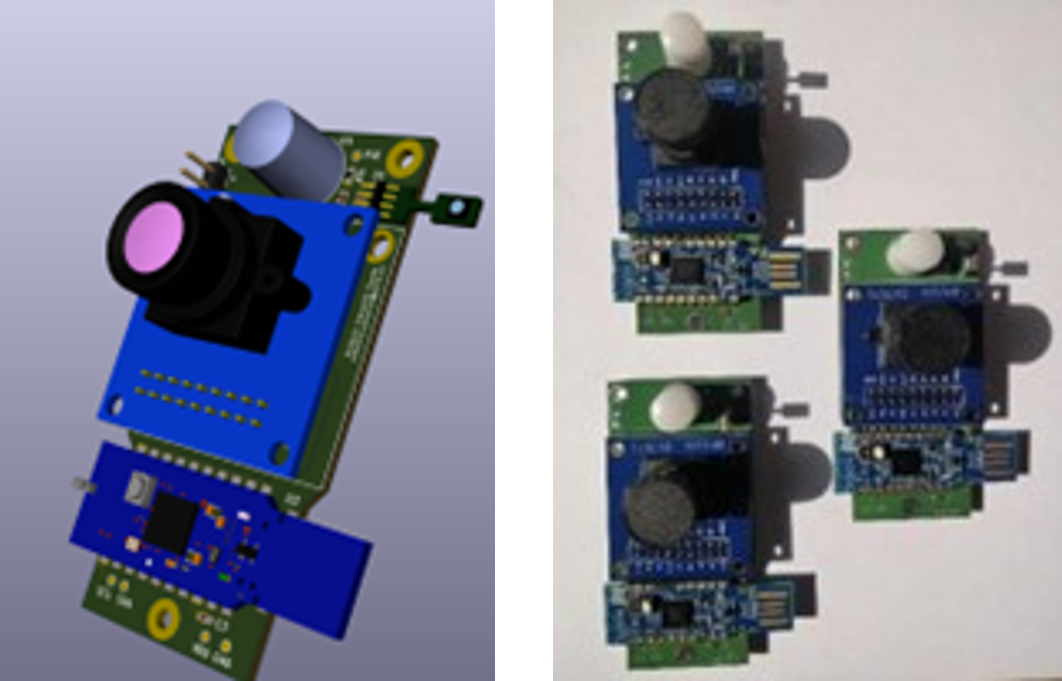
\includegraphics[width=0.6\linewidth]{images/SensorNodes.png}
	\caption{AI\_r Sensor Nodes}
	\label{fig:SensorNodes}
\end{figure}


\begin{figure}[ht]
	\centering
	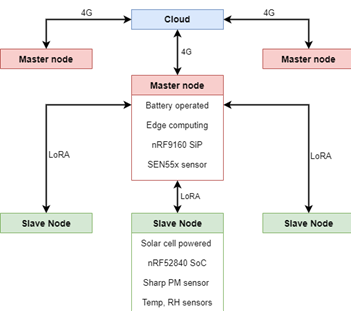
\includegraphics[width=0.5\linewidth]{images/Network_topology_of_AI_r_system_cropped.png}
	\caption{Network Topology of AI\_r System}
	\label{fig:NetworkTopology}
\end{figure}



\subsection{Wireless Communication}
[Wireless communication methods used in the system are...]
\subsubsection{LoRa}

\begin{figure}[ht]
	\centering
	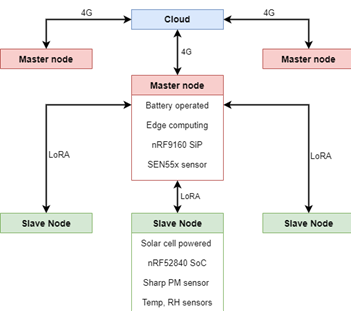
\includegraphics[width=0.5\linewidth]{images/Network_topology_of_AI_r_system_cropped.png}
	\caption{Network Topology of AI\_r System}
	\label{fig:NetworkTopology}
\end{figure}

Text \Cref{fig:LoRaTransmissionSpectogram}

\begin{figure}[ht]
	\centering
	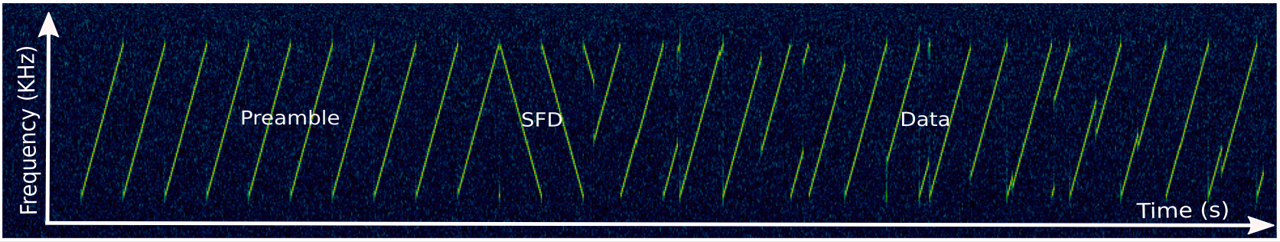
\includegraphics[width=0.8\linewidth]{images/LoRa transmission spectogram.png}
	\caption{Spectogram of LoRa Transmission, taken from \cite{Liando2019KnownStudy}}
	\label{fig:LoRaTransmissionSpectogram}
\end{figure}


\begin{enumerate}
    \item Network Topologies
    \item Performance Metrics
\end{enumerate}

\subsubsection{4G}
\begin{enumerate}
    \item Network Analysis
    \item Performance Metrics
\end{enumerate}

\subsection{Mining Environment}
\subsubsection{Typical Mining Architectures}
\subsubsection{Network Interference in Mining Context}

\section{Related Work}

\section{Conclusion}

\chapter{Research Aims, Hypothesis and Methodology}
[The candidate shows a familiarity with the
methods available for solving the research
problem or answering the research question,
and the chosen methods are well-motivated.]

\section{Problem Statement}
\section{Research Question}
[The research problem or question is clear, sufficiently narrow, and solvable or answerable
within the constraints of the project.]
\section{Research Aims and Objectives}
\subsection{Research Aims}
[The aim and objectives are relevantly related
to the research problem or question.]
\subsection{Objectives}
\section{Limitations}
\begin{itemize}
\item Apparatus
\item Mine context
\end{itemize}

\section{Research design}
\section{Methods}
\section{Limitations}

\chapter{Schedule of Work}
[The schedule of work is sufficiently detailed
and is feasible
]
\section{Schedule of Work}


\chapter{Latex tools}

\section{A Section about Citation Style}
Citations are important. Citation style for Computer Science is:
\begin{itemize}
\item When used in the text, use the authors with the date in brackets:\\ \citet{klein17} say very important things.
\item When used as a reference after a face, put everything in brackets:\\ Import things are true \citep{klein17}.
\end{itemize}

\section{Compiling}
Remember to compile multiple times to resolve references. Usually:
\begin{verbatim}
pdflatex file.tex
bibtex file
pdflatex file.tex
pdflatex file.tex
\end{verbatim}


\LaTeX\ decides how to place images. It also does the referencing for you as seen in \Cref{fig:thing1}. If you have subimages, they should have their own captions and labels -- look into the subfig or subfigure packages.

\begin{figure}[ht]
	\centering
	
\includegraphics[width=0.1\linewidth]{images/wits}
	\caption{This is an image}
	\label{fig:thing1}
\end{figure}

Figure captions are at the bottom. Table title are at the top of the table as seen in \Vref{tab:tab1}. There is a package called BookTabs which is \textit{way} better for tables and you should learn how to use that instead.

\begin{table}[p]
	\centering
	\caption{Table Name}
	\label{tab:tab1}
\begin{tabular}{cc}
	\hline
	Col1 & Col2\\
	\hline\hline 
	R0,C0 & R0,C1 \\ 
	R1,C0 & R1,C1 \\ 
	\hline
\end{tabular} 
\end{table}

Usually let \LaTeX\ handle the placement of floats unless you \textit{really} need to force it to do something else. The \texttt{float} package used above allows you to use \texttt{H} as the placement which means \textit{here and only here}. When using the float package, the placement options are:
\begin{enumerate}
\item h -- a gentle nudge to place it here if possible
\item t -- top of a page
\item b -- bottom of a page
\item H -- here and only here, do not move it at all
\item p -- on its own page
\end{enumerate}


\chapter{Some Referencing Tricks}
CleverRef and VarioRef are helpful:
\begin{itemize}
	\item Normal Ref: See Figure \ref{fig:thing1}
	\item CleverRef: See \Cref{fig:thing1} and \Cref{tab:tab1}
	\item CleverRef+VarioRef: See \Vref{fig:thing1} and \Vref{tab:tab1}
\end{itemize}


\appendix
\chapter{Extra Stuff}\label{app:extra}
\section{What is an appendix?}\label{app:whatis}

An appendix is useful when there is information that you need to include, but breaks the flow of your document, e.g. a large number of figures/tables may need to be shown, but maybe only one needs to be in the text and the rest are just included for completeness.

\nocite{*}

\bibliography{references, references-mendeley}\addcontentsline{toc}{chapter}{References}
\end{document}
